\documentclass{beamer}
\usepackage[latin1]{inputenc}
\usepackage{graphicx}
\usepackage{amsmath}
\usepackage{verbatim}
\usepackage{listings}
\usepackage{color}
\usetheme{Frankfurt}

\def\Tiny{\fontsize{4pt}{4pt}\selectfont}

\begin{document}

\usebackgroundtemplate
{

\includegraphics[height=\paperheight,width=\paperwidth]{pic/esrf_crisp/esrf_crisp_default.jpeg}
}

\begin{frame}{CRISP 2nd annual meeting}
\begin{center}
The use of hardware virtualization in RASHPA
\end{center}
\end{frame}

\setbeamertemplate{items}[circle]
\begin{frame}{Contents}
  \begin{itemize}
  \item RASHPA context reminder
  \item Device virtualization
  \item The VPCIe framework
  \end{itemize}
\end{frame}

\begin{frame}{Context - RASHPA reminder}
  \begin{center}
    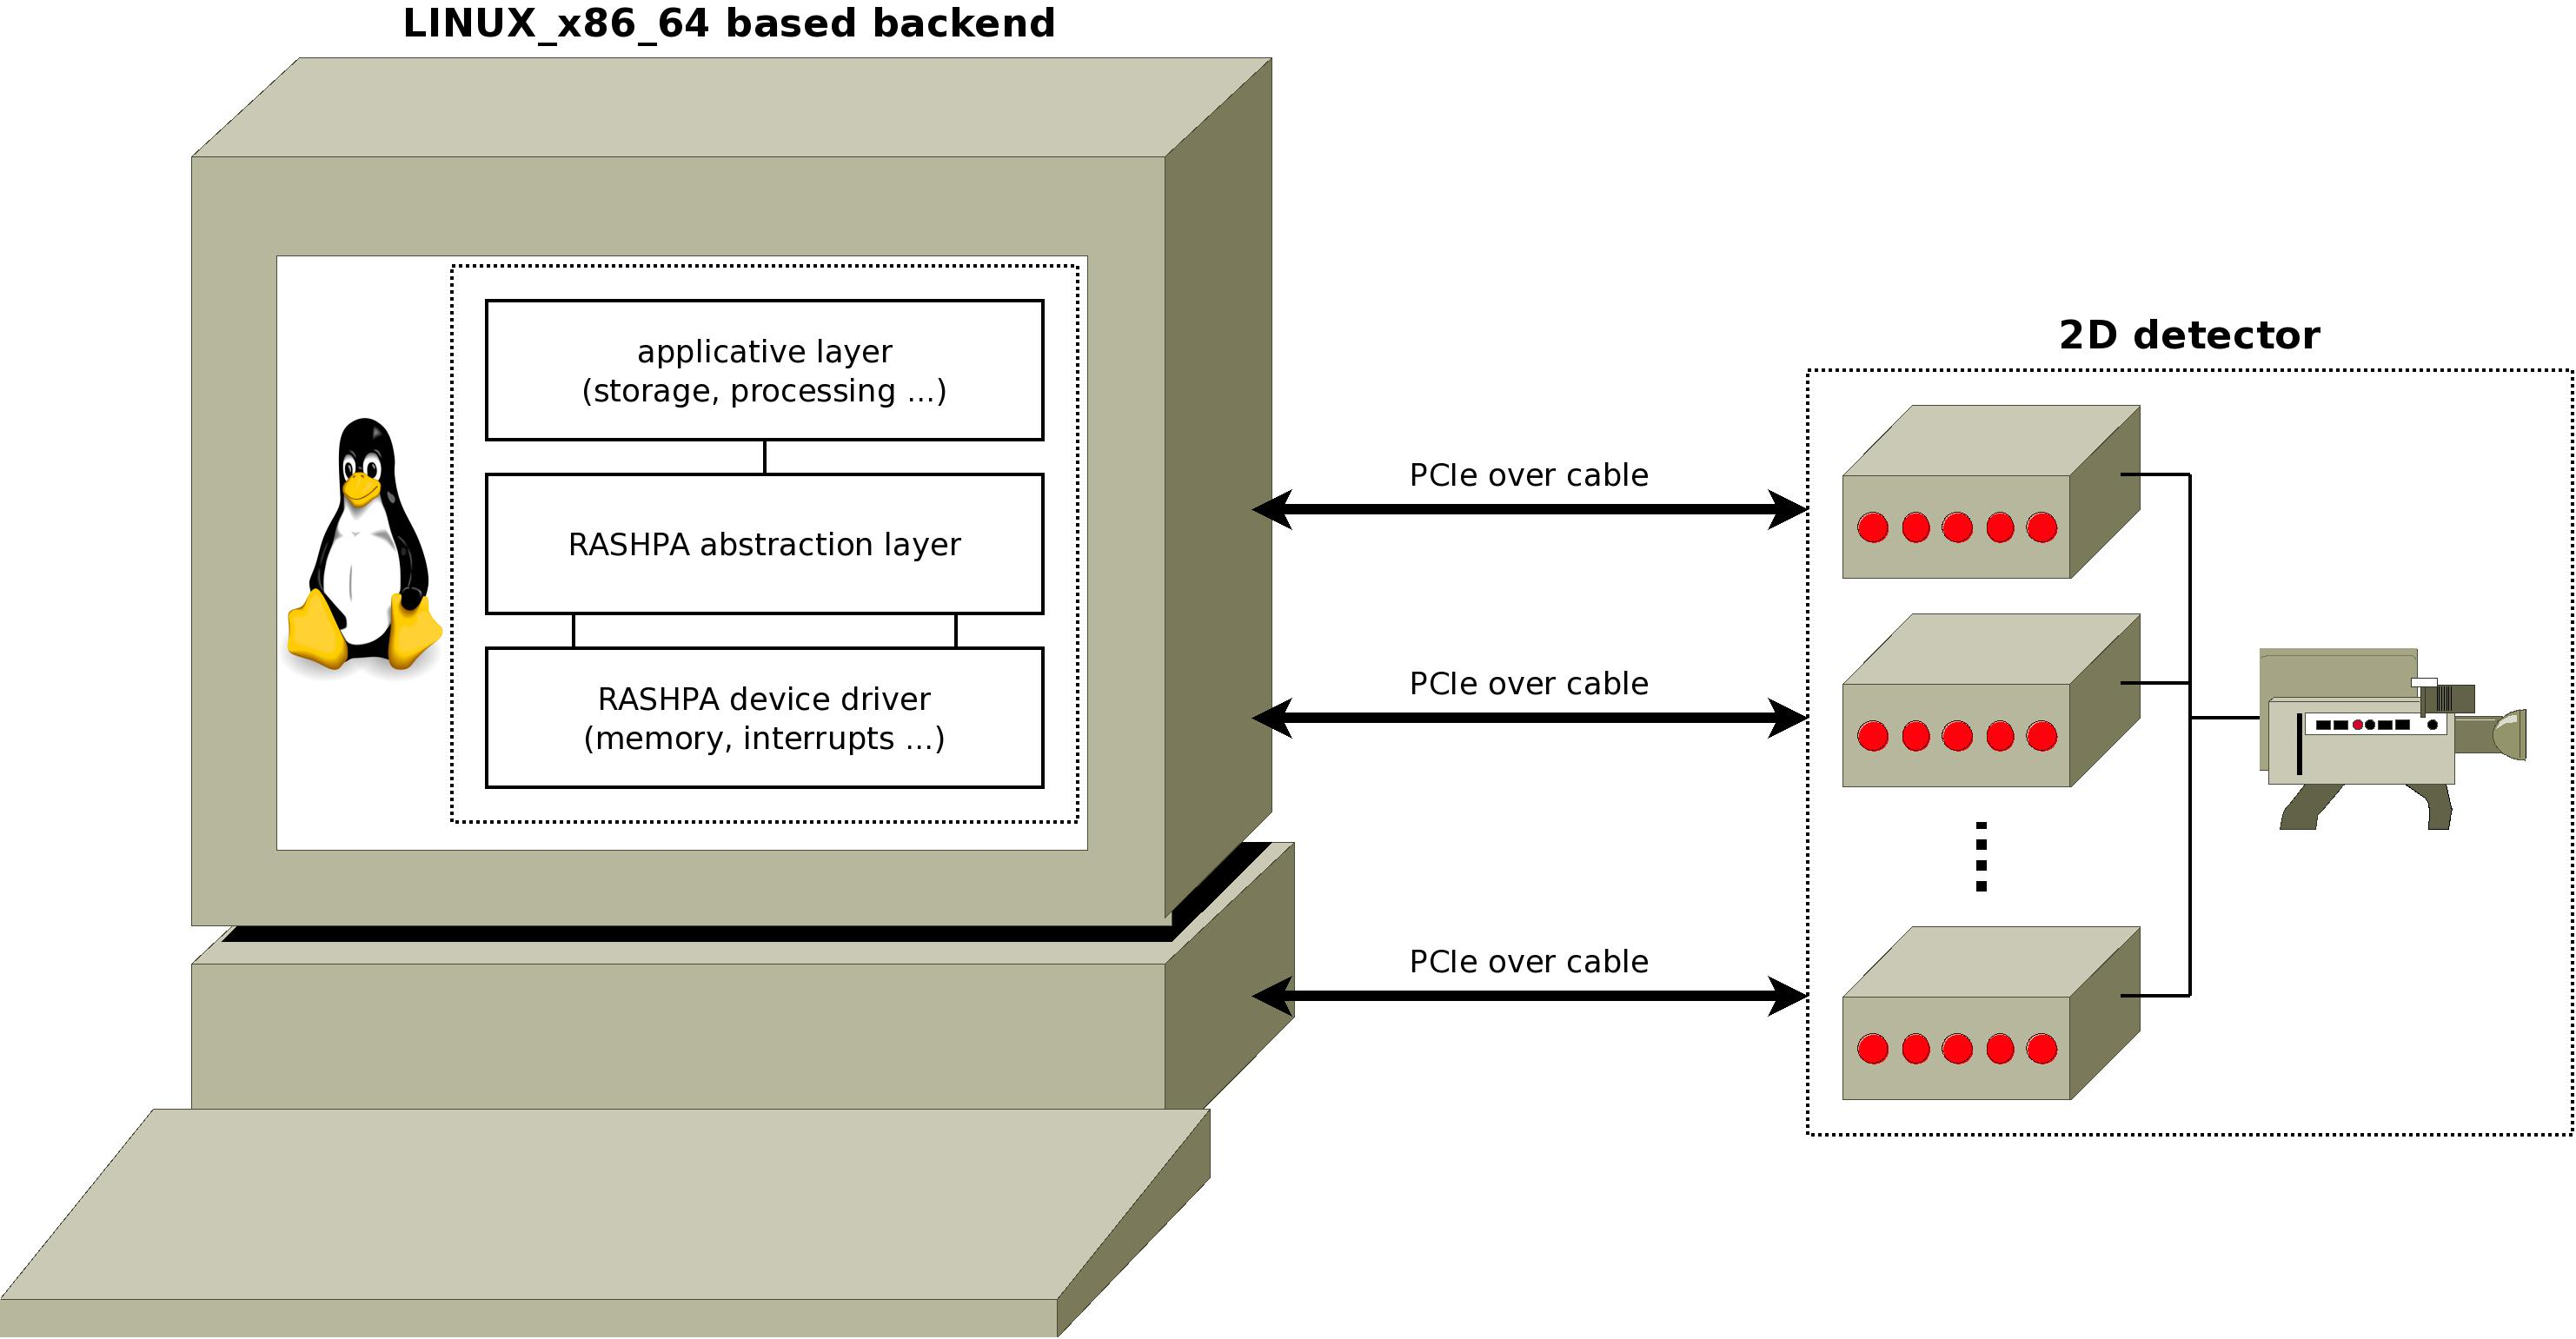
\includegraphics[width=75mm]{pic/dv_reminder/main.jpeg}
  \end{center}
  \begin{tiny}
  RASHPA basic goal is to transfer \textbf{detector} memory contents into
  a \textbf{backend} for further processing, visualisation or storage. To
  do so, RASHPA relies on low level hardware and software components:\\
  \begin{itemize}
  \item data \textbf{transport layer}, currently PCI Express over cable
  \item a data \textbf{transmission engine} implemented on XILINX FPGA
  \item a LINUX \textbf{software stack}, ie. kernel device driver and applications
  \end{itemize}
  \end{tiny}
\end{frame}

\begin{frame}{Context - RASHPA project issues}
  \begin{small}
  Still being prototyped
  \begin{itemize}
  \item how to simplify hardware software \textbf{codesign} ?
  \end{itemize}

  Aims at using multiple PCIe links. Yet, the first prototype is single link
  \begin{itemize}
  \item how to \textbf{scale} the prototype platform ?
  \end{itemize}

  Well positionned to interface with PCIe based accelerating technologies
  \begin{itemize}
  \item how to test \textbf{unavailable hardware} (too recent or expensive) ?
  \end{itemize}
  \end{small}
\end{frame}

\begin{frame}{Context - Our approach}
  \begin{center} Our approach: \textbf{device virtualization} \end{center}
\end{frame}

\begin{frame}{Device virtualization - main idea}
  \begin{center}
    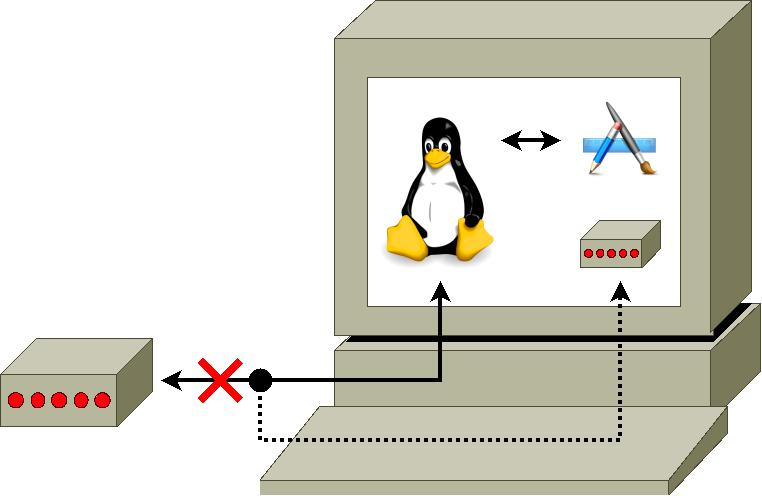
\includegraphics[width=45mm]{pic/dv_redirect/main.jpeg}
  \end{center}
  \begin{small}
    Applications on a \textbf{host} machine access hardware via interfaces. By
    \textbf{instrumenting} these interfaces, one can \textbf{redirect} the accesses
    to a software implementing the device. The device is said to be
    \textbf{virtualized}.
  \end{small}
\end{frame}

\begin{frame}{Device virtualization - assumptions}
  \begin{small}
  Virtualization assumes device accesses are made using a known interface
  \begin{itemize}
  \item software library API (system calls)
  \item memory mapped registers
  \item CPU specific instructions (in, out)
  \end{itemize}
  \end{small}
\end{frame}

\begin{frame}{Device virtualization - mechanisms}
  \begin{small}
  The interface is then instrumented to redirect access to the virtual device
  \begin{itemize}
  \item software hooking (code instrumentation, library replacing)
  \item \textbf{instruction emulation (QEMU)}
  \item hardware traps (page protection)
  \item architecture support (INTEL VT)
  \item paravirtualization (XEN)
  \end{itemize}
  \end{small}
\end{frame}

\begin{frame}{Device virtualization - applications}
  Device virtualization example applications
  \begin{itemize}
  \item support: application running on unmaintained platform
  \item security: sandboxing, reverse engineering
  \item quality: debugging, fault injection
  \item testing: milkymist, zinq, android
  \end{itemize}
\end{frame}

\begin{frame}{VPCIe - introduction and goals}
  VPCIe: a framework to virtualize PCIe devices
  \begin{itemize}
  \item made at the ESRF in the context of CRISP/RASHPA
    \setbeamertemplate{items}[triangle]
    \begin{itemize}
    \item still, generic enough to fit other project needs
    \end{itemize}
    \setbeamertemplate{items}[circle]
  \item the backend software must run \textbf{without any modification}
  \item virtual device implementation usable in the real device
    \setbeamertemplate{items}[triangle]
    \begin{itemize}
    \item made possible with \textbf{VHDL}
    \end{itemize}
    \setbeamertemplate{items}[circle]
  \end{itemize}
\end{frame}

\begin{frame}{VPCIe - opensource building blocks}
  VPCIe mostly relies on opensource projects
  \newline

  \textbf{QEMU}
  \begin{itemize}
  \item http://wiki.qemu.org/Main\_Page
  \item architecture emulator (X86\_64, ARM ...)
  \item used to trap PCIe hardware accesses
  \end{itemize}

  \textbf{GHDL}
  \begin{itemize}
  \item http://ghdl.free.fr
  \item VHDL frontend for GCC
  \item used to implement device in VHDL
  \end{itemize}

\end{frame}

\begin{frame}{VPCIe - implementation}
  \begin{center}
  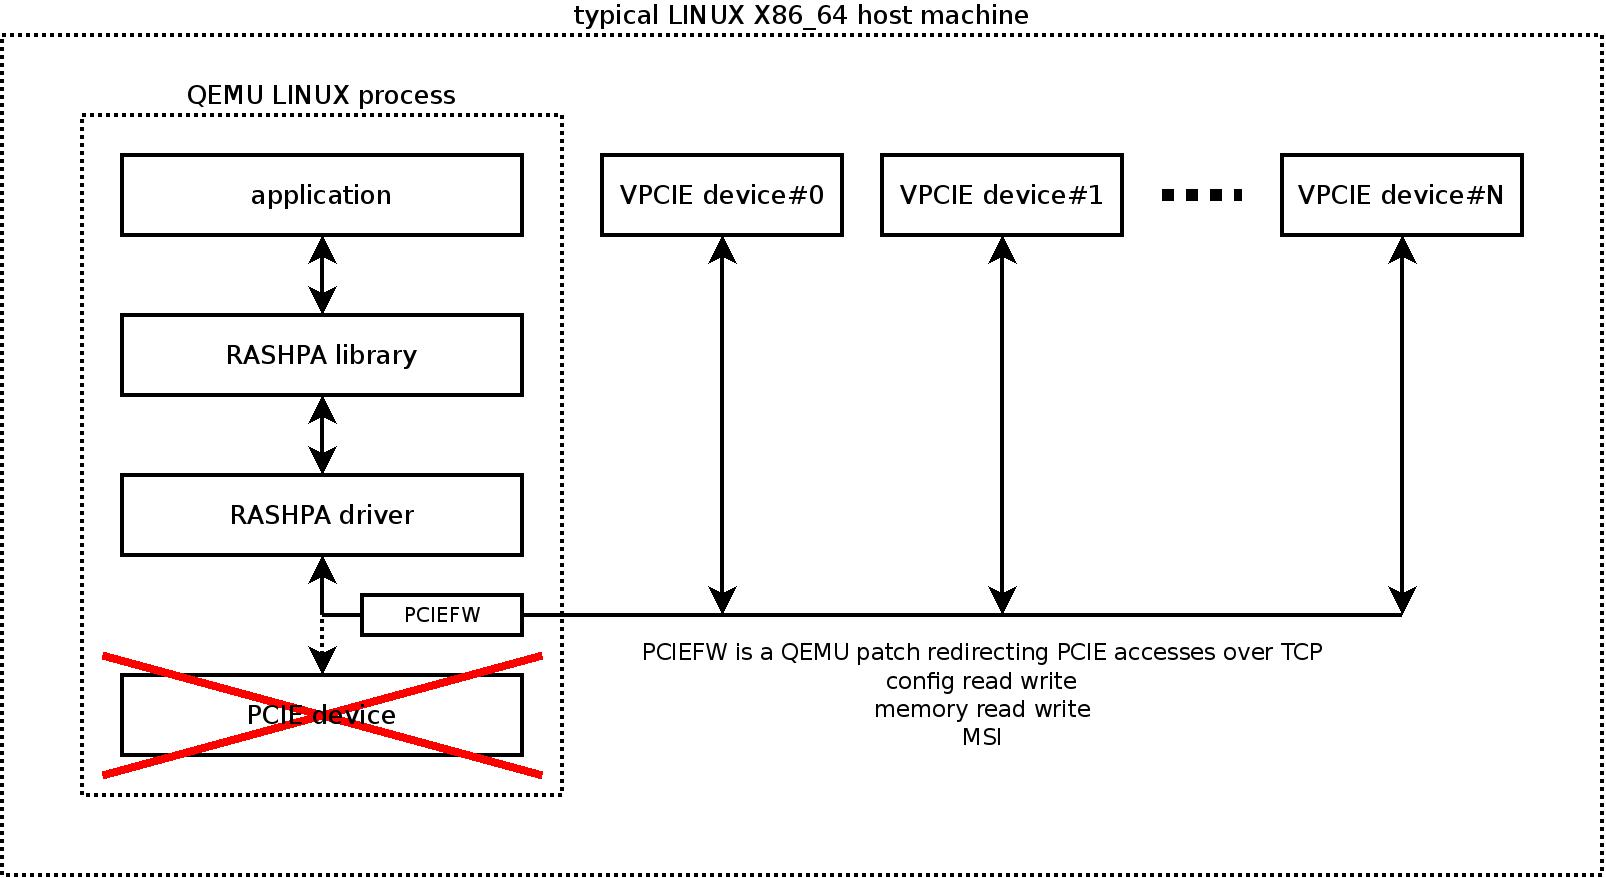
\includegraphics[width=80mm]{pic/dv_implem/main.jpeg}
  \end{center}
\end{frame}

\begin{frame}{VPCIe - RASHPA possible setup}
  \begin{center}
  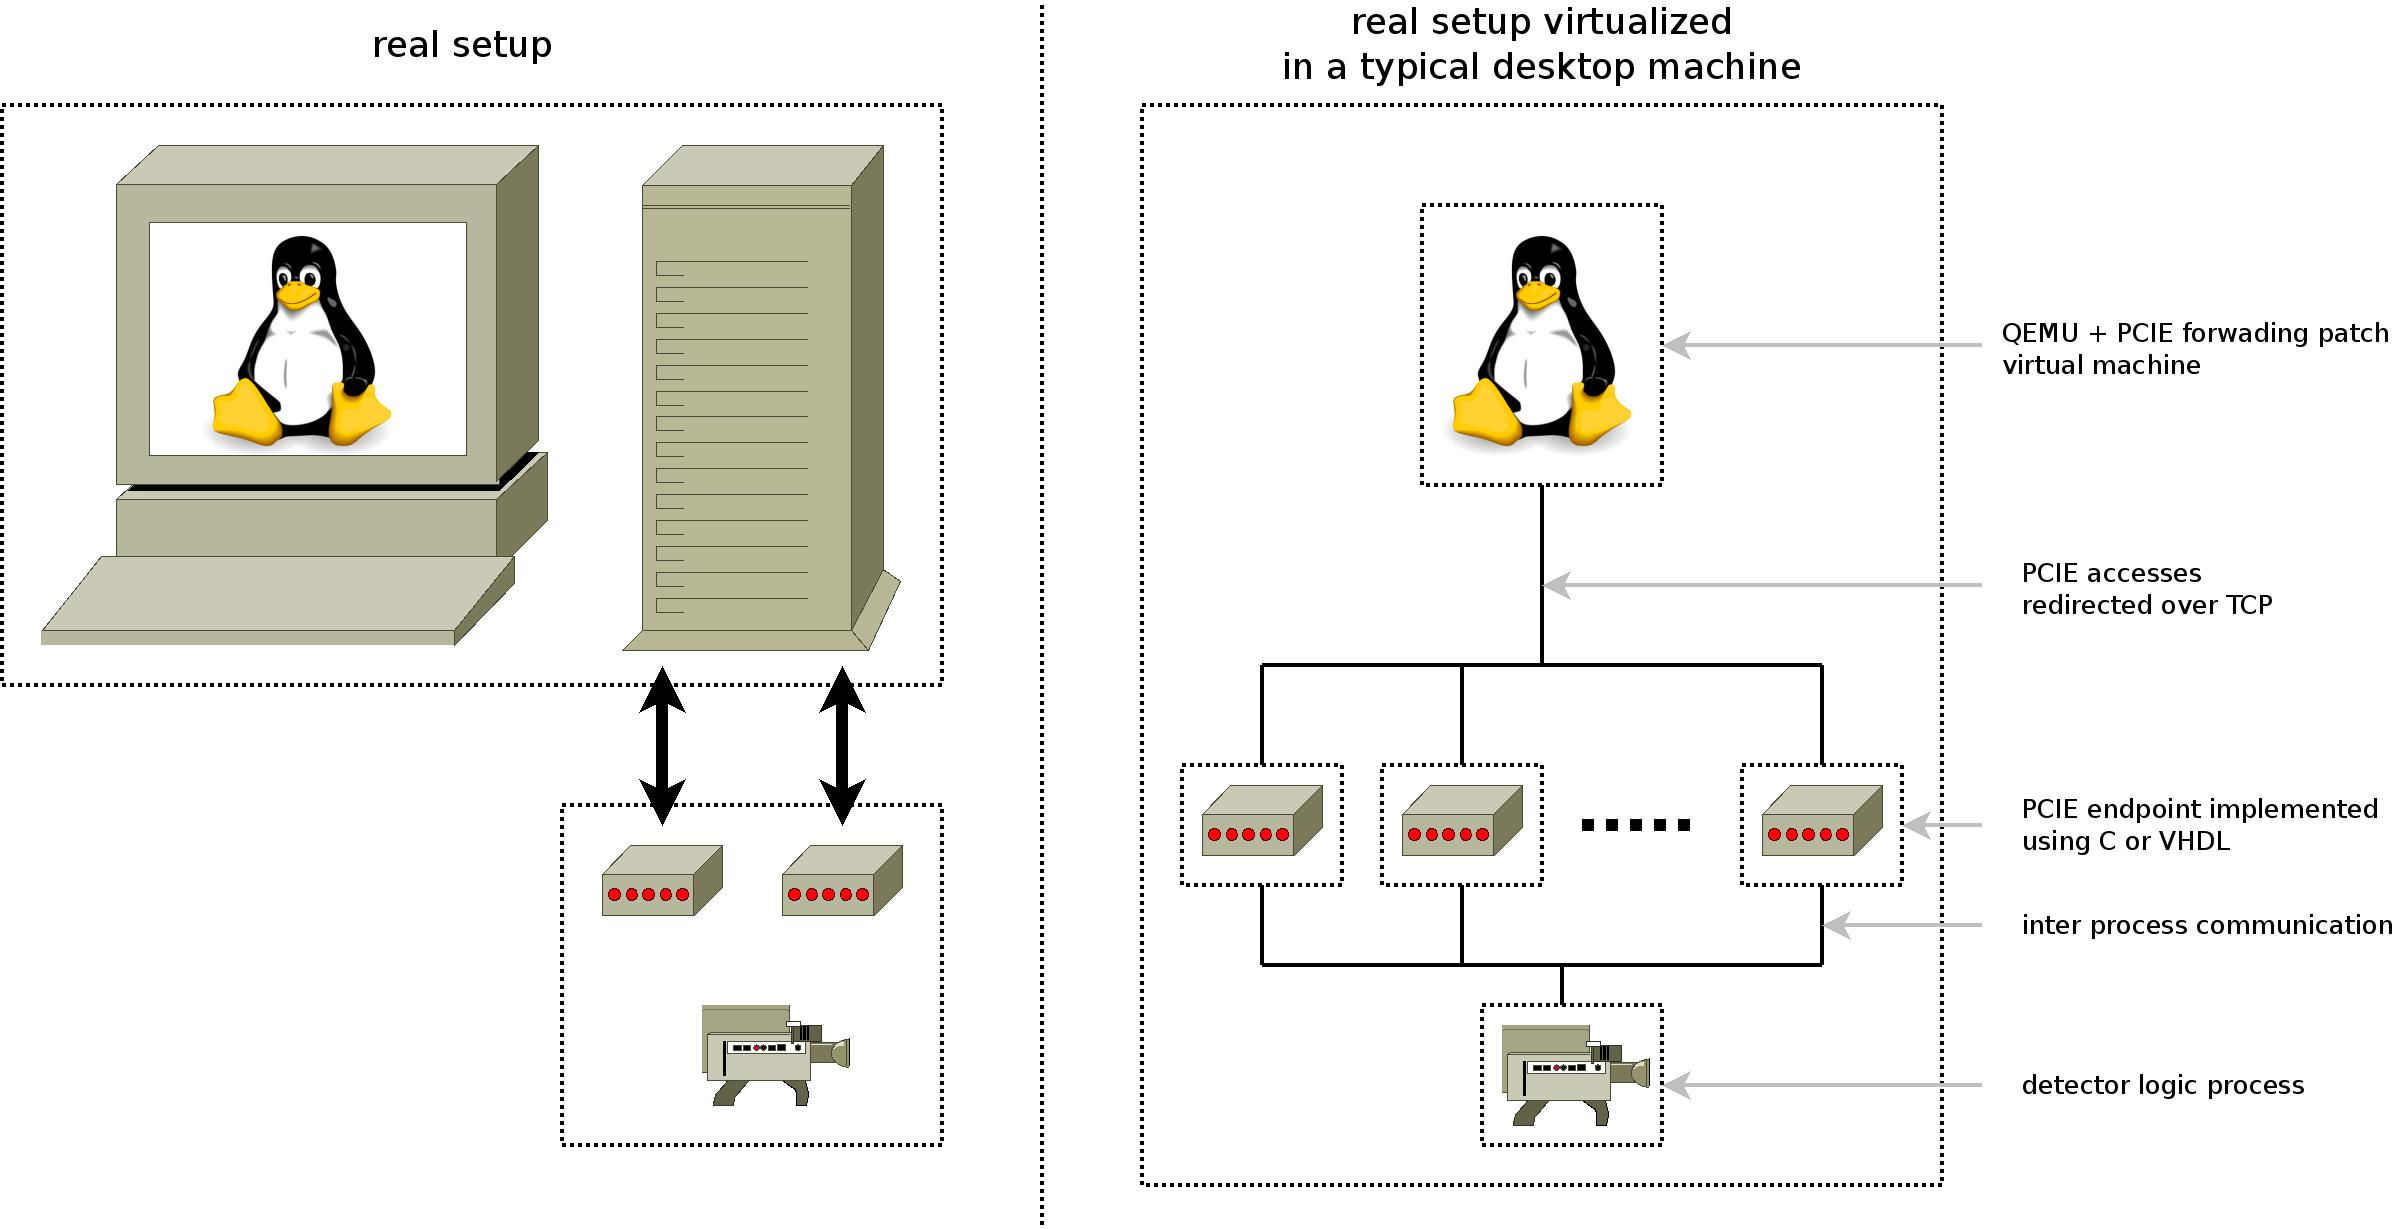
\includegraphics[width=80mm]{pic/dv_vpcie/main.jpeg}
  \end{center}
\end{frame}

\begin{frame}{VPCIe - RASHPA backend}
  RASHPA backend is a full featured LINUX system
  \begin{itemize}
  \item runs in a QEMU virtual machine
  \item PCIe accesses are trapped and sent over TCP to the devices
  \item PCIe forwarder is available as a QEMU patch
    \setbeamertemplate{items}[triangle]
    \begin{itemize}
    \item discussions in progress for a merge
    \end{itemize}
    \setbeamertemplate{items}[circle]
  \end{itemize}
\end{frame}

\begin{frame}{VPCIe - RASHPA emulated devices}
  RASHPA emulated devices
  \begin{itemize}
  \item run as a LINUX processes, can be \textbf{duplicated} at will
  \item can be implemented in \textbf{C} or \textbf{VHDL}
  \item PCIe made \textbf{simple}, focus on device logic
  \end{itemize}
\end{frame}

\begin{frame}[containsverbatim]
 \frametitle{VPCIe - emulated device VHDL interface}
 \begin{tiny}
 \lstset{commentstyle=\color{blue}}
 \lstset{language=VHDL}
 \begin{lstlisting}[frame=tb]
entity endpoint is
 port
 (
  rst: in std_ulogic;
  clk: in std_ulogic;

  req_en: out std_ulogic;
  req_wr: out std_ulogic;
  req_bar: out std_ulogic_vector(pcie.BAR_WIDTH - 1 downto 0);
  req_addr: out std_ulogic_vector(pcie.ADDR_WIDTH - 1 downto 0);
  req_data: out std_ulogic_vector(pcie.DATA_WIDTH - 1 downto 0);

  rep_en: in std_ulogic;
  rep_data: in std_ulogic_vector(pcie.DATA_WIDTH - 1 downto 0);

  mwr_en: in std_ulogic;
  mwr_addr: in std_ulogic_vector(pcie.ADDR_WIDTH - 1 downto 0);
  mwr_data: in std_ulogic_vector(pcie.PAYLOAD_WIDTH - 1 downto 0);
  mwr_size: in std_ulogic_vector(pcie.SIZE_WIDTH - 1 downto 0);

  msi_en: in std_ulogic
 );
end entity;
 \end{lstlisting}
 \end{tiny}
\end{frame}

\begin{frame}[containsverbatim]
 \frametitle{VPCIe - emulated device C interface}
 \begin{tiny}
 \lstset{commentstyle=\color{blue}}
 \lstset{language=C}
 \begin{lstlisting}[frame=tb]

/* runtime initialization */
int pcie_init_net(pcie_dev_t*, ...);
int pcie_fini(pcie_dev_t*);
int pcie_loop(pcie_dev_t*);

/* misc config byte accessors */
int pcie_set_deviceid(pcie_dev_t*, ...);
int pcie_set_vendorid(pcie_dev_t*, ...);

/* PCIe BAR access handlers */
typedef void (*pcie_readfn_t)(uint64_t, void*, size_t, void*);
typedef void (*pcie_writefn_t)(uint64_t, const void*, size_t, void*);
int pcie_set_bar(pcie_dev_t*, ..., pcie_readfn_t, pcie_writefn_t, ...);

/* host memory read write operations */
int pcie_write_host_mem(pcie_dev_t*, uint64_t, size_t*);
int pcie_read_host_mem(pcie_dev_t*, uint64_t, size_t*);

/* send an MSI */
int pcie_send_msi(pcie_dev_t*);
 \end{lstlisting}
 \end{tiny}
\end{frame}

\begin{frame}{VPCIe - tested to virtualize ESRF prototyping plateforms}
  \begin{center}
  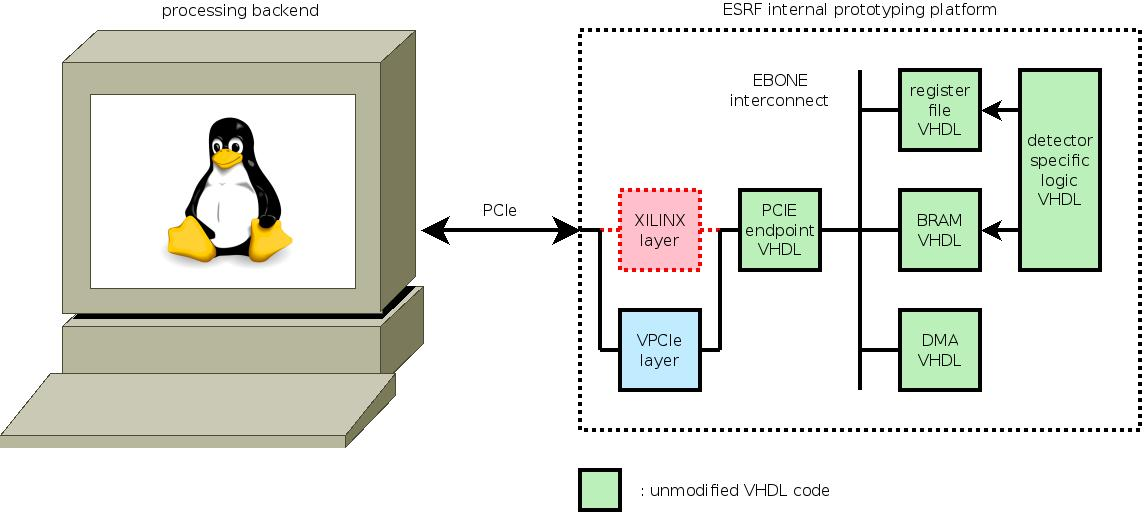
\includegraphics[width=80mm]{pic/dv_ebone/main.jpeg}
  \end{center}
\end{frame}

\begin{frame}{VPCIe - benefits}
  Hardware software codesign
  \begin{itemize}
  \item reduce development time
  \item no \textbf{modification} on the backend software (esp. driver)
  \item act as a stimuli generator for VHDL simulations
  \end{itemize}

  Platform scaling
  \begin{itemize}
  \item one PCIe endpoint per LINUX process
  \end{itemize}

  Investigate unavailable technologies
  \begin{itemize}
  \item NVM Express support for QEMU is available
  \end{itemize}
\end{frame}

\begin{frame}{VPCIe - more benefits}
  Virtual machine
  \begin{itemize}
  \item resources easily changed (RAM amount ...)
  \item test with different CPU architectures (x86, x86\_64, ARM ...)
  \item small LINUX disk images reduce reboot times (few seconds)
  \end{itemize}
  Fault injection
  \begin{itemize}
  \item LINUX and software response to PCIe device disconnection
  \end{itemize}
\end{frame}

\begin{frame}{VPCIe - availability}
  VPCIe source is available online
  \begin{itemize}
  \item https://github.com/texane/vpcie
  \item documentation still poor, but clear examples
  \item feedbacks or contributions are welcome
  \end{itemize}
\end{frame}

\begin{frame}{VPCIe - questions}
  \begin{center} Thanks for your attention. \end{center}
  \begin{center} Feel free to ask for a demo after the talk. \end{center}
  \begin{center} Any question? \end{center}
\end{frame}

\end{document}
